\chapter{Project Management\label{chap3}}
This chapter is about the management skills employed during the development. We first introduce our division of work as a result of the Statement of Work and the Work Breakdown Structure. The development strategy is also discussed in this section. To enhance the work efficiency, we utilize two online platforms, ZenHub and GitHub, for the schedule management and version control respectively.
\section{Division of Work}
In order to divide the project into achievable tasks and assign tasks to the most suitable team member, the first step of the project management is to do the Task Orientation so that the requirements are able to be achieved efficiently and completely. 

In the part of task orientation, we have strictly obeyed the process of the project management. First of all, the Statement of Work (SoW) is made to convert the whole project into realistic and achievable goals. Also, it has the function of establishing expectation of the final result. On top of the SoW, a Work Breakdown Structure (WBS) is needed to divide the whole team into several groups. The function of the WBS is to figure out all the works required to be done to complete the project and structure the work into logic components and subcomponents. The individual responsibilities can also be assigned. 

\begin{figure}[htbp]
    \centering
    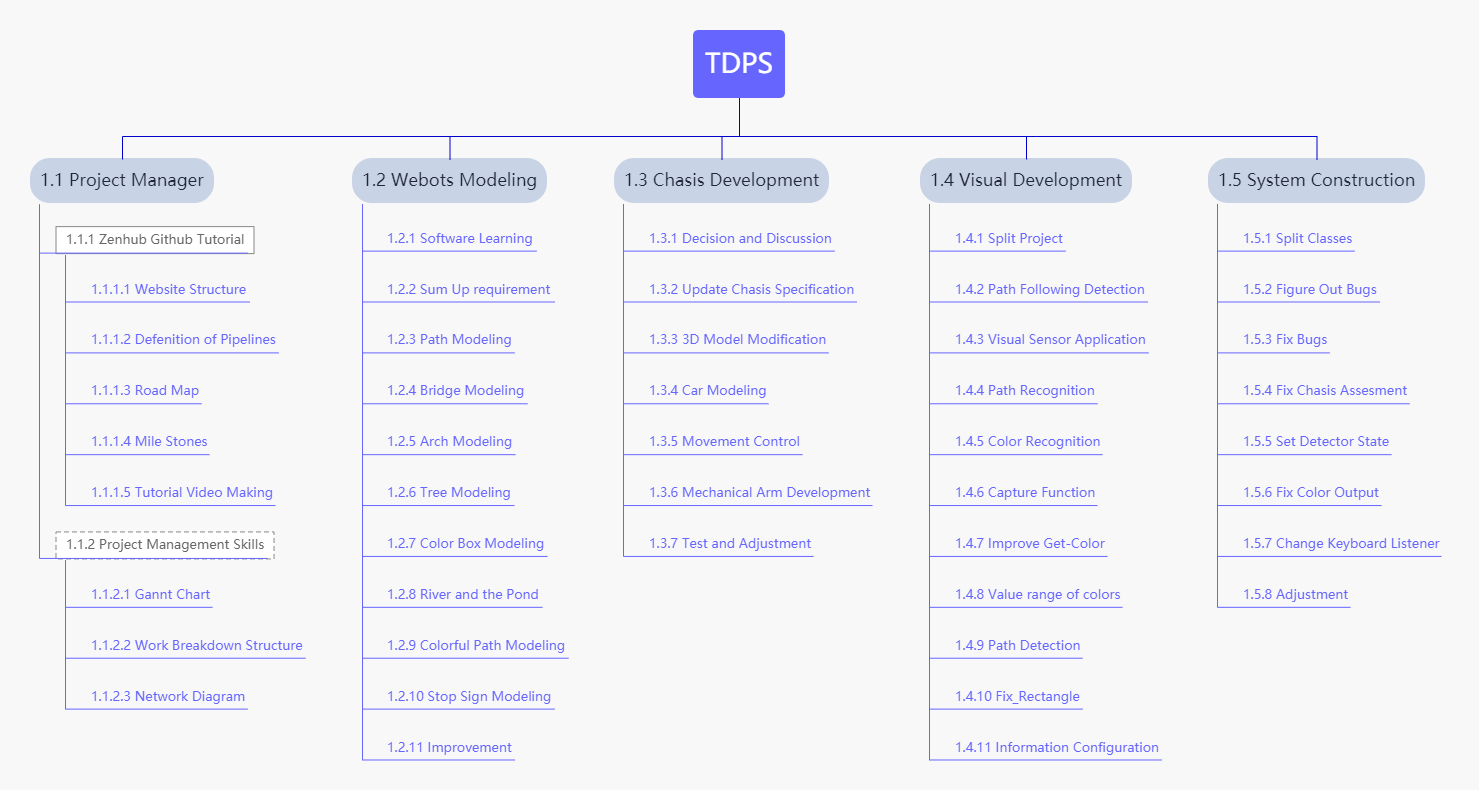
\includegraphics[width=14cm]{management/img_management/WBS.png}
    \caption{The Work Breakdown Structure}
    \label{fig:WBS}
\end{figure}

Our WBS is shown in Figure \ref{fig:WBS}. According to it, we form 5 technical subgroups, including the Environment Group, the Visual Group, the Decision Group, the Chassis Group and the System Group, and one Documentation Group. In addition, we assign a project manager and a tech leader to take responsible for progress control and tech support. For a detailed version of personnel division and individual contribution, please refer to the Appendix \ref{appendix}.
%-----------------------------------------------------------------------
\section{Schedule Management \& Version Control}
\subsection{Schedule Management}
Due to the outbreak of the COVID-19, this project is forced to be finished online this year. Hence, reasonable scheduling to track the progress of the whole project becomes an indispensable part of the project management. ZenHub is an excellent web application for team work, on which we decide to base the development of our project. Figure \ref{fig:ZenHub} is a screenshot of the ZenHub board, which is made up of seven pipelines. They are New Issues, Epics, Help Wanted, In Progress, Backlog, Bugs and Closed. 

\begin{figure}[htbp]
    \centering
    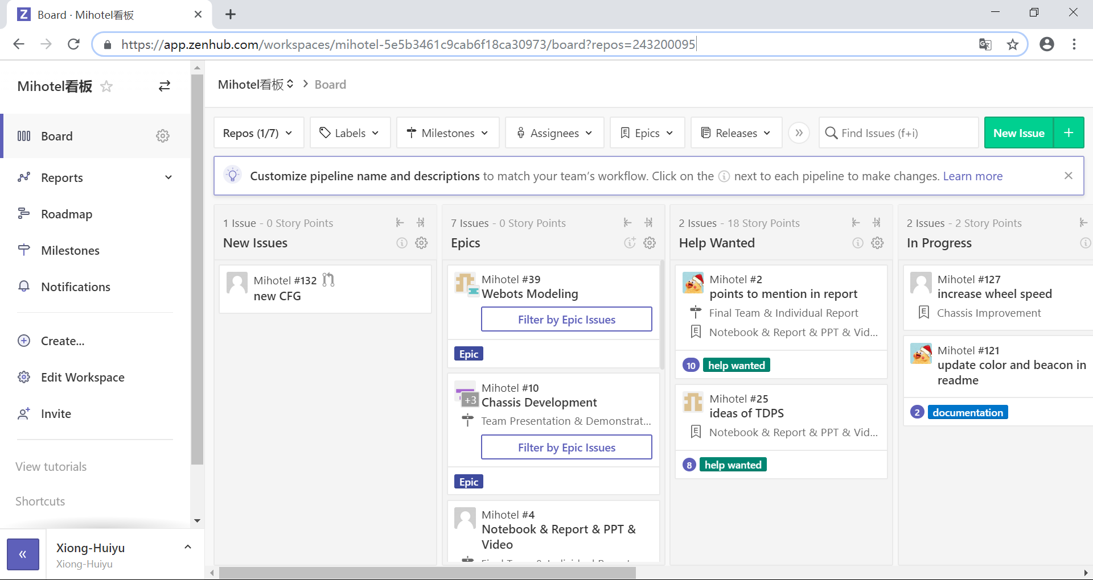
\includegraphics[width=14cm]{management/img_management/ZenHub.png}
    \caption{The user interface of ZenHub}
    \label{fig:ZenHub}
\end{figure}

ZenHub Pipelines are built on the basis of GitHub repositories and each "card" on the Board represents a GitHub Issue or Pull Request. Once a issue is newly created, it will appear immediately in the New Issues pipeline before moved to other regions. ZenHub Epics bundle similar groups of Issues together, providing a visual progress bar of work across related or dependent Issues. This panel can be regarded as a group panel, each group will have their own Epic panel containing their design tasks. After it follows the Help Wanted, which consists of  problems requiring suggestions or solution from each member of the team. The next pipeline is In Progress, indicating that someone in the team is dealing with issues or pull requests inside it. The Backlog pipeline contains issues needing to be completed before the end of the project but not of the highest priority at present, or not able to be done without enough accumulation. After one issue is finished, it goes directly into the Closed pipeline. Team members can browse this pipeline to check what they have done so far or reopen specific issues if they find some problems with these issues later on.

Another important feature of ZenHub is the Roadmap, which is a in-built Gantt Chart automatically generated by ZenHub. As we discuss before, ZenHub groups issues using Epics. For example, issues proposed by the Visual Group are all tagged the Visual Development Epic. As is shown in Figure \ref{fig:roadmap}, different epics are represented by blocks of distinct colors. When creating a issue, we need to set the estimate time to finish it. Thus, the length of each colored block stands for the sum of estimate time of all issues in this epic. The black line in each colored block tracks how many issues are resolved within this epic. If no issue is left, the black line will have the same length as the colored block. The Roadmap is beneficial to our schedule management. We effectively track our progress by checking whether the black line in each epic is aligned with today's date. In short, the Roadmap contributes a lot to our schedule management, offering a broad picture about the project progress.

\begin{figure}[htbp]
    \centering
    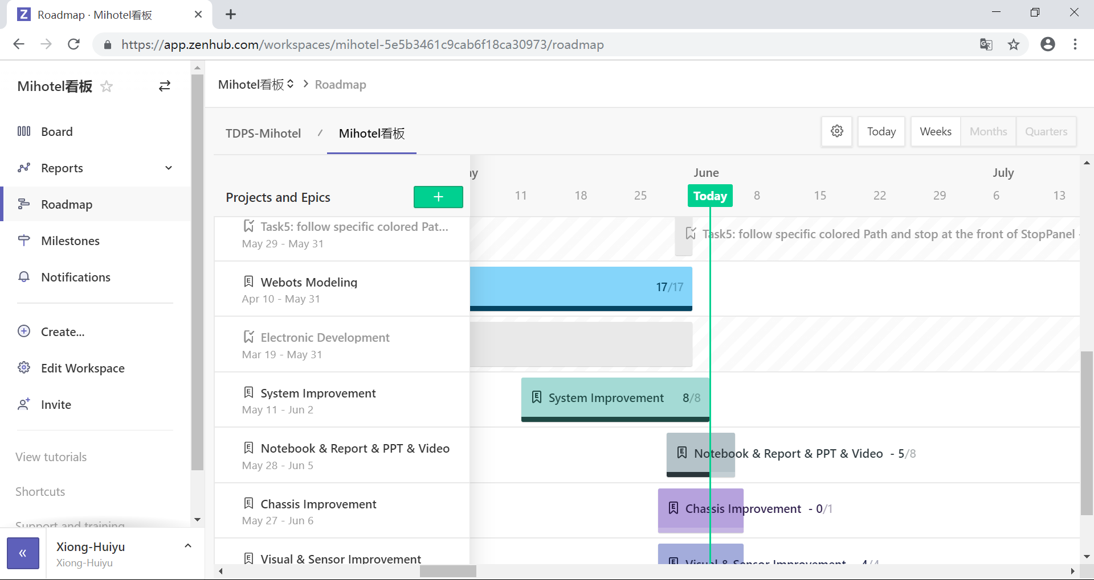
\includegraphics[width=14cm]{management/img_management/Roadmap.png}
    \caption{Roadmap: A simpler version of the Gantt Chart on ZenHub}
    \label{fig:roadmap}
\end{figure}

\subsection{Version Control}
During team development, another frequently occurring problem is the version conflict. Supposing two team members are editing the same program, chances are that the one of them is unaware of changes made by the other. In that case, the code will not work if they directly merge two programs together. What's more, it is also time-consuming for people to merge codes manually. With an attempt to avoid this problem, we base our development process on GitHub.

There are two key benefits of using GitHub. One is the discussion board within each issue, which provides us with a unique platform to communicate with team member. The other is the Pull Request. Figure \ref{fig:request} illustrates the use of Pull Request. The black line on the top represents the master branch, which is the base version of our codes. In order to tackle different issues independently, several branches are created. They are the colored lines in Figure \ref{fig:request}. Once the assignees solve issues in each branch, request will be pulled to merge this branch into the master. Reviewers are responsible to check if their requests really fix the problem.

\begin{figure}[htbp]
    \centering
    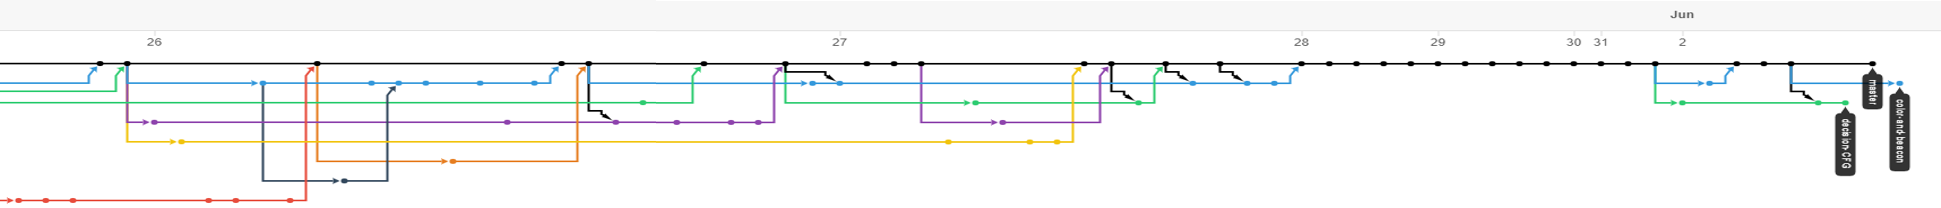
\includegraphics[width=15cm]{management/img_management/version_control.png}
    \caption{Requests merged into the master branch}
    \label{fig:request}
\end{figure}

As we mention before, the issues can be viewed as small cards in different pipelines on ZenHub. Similar to cards, we can write our ideas on them. Figure \ref{fig:issue}
takes one issue during our development as an example. It share the same strength as the E-mail, keeping important dialog between team members. If someone want to check some details about the design, he can find corresponding notes easily in this discussion board.
\begin{figure}
    \centering
    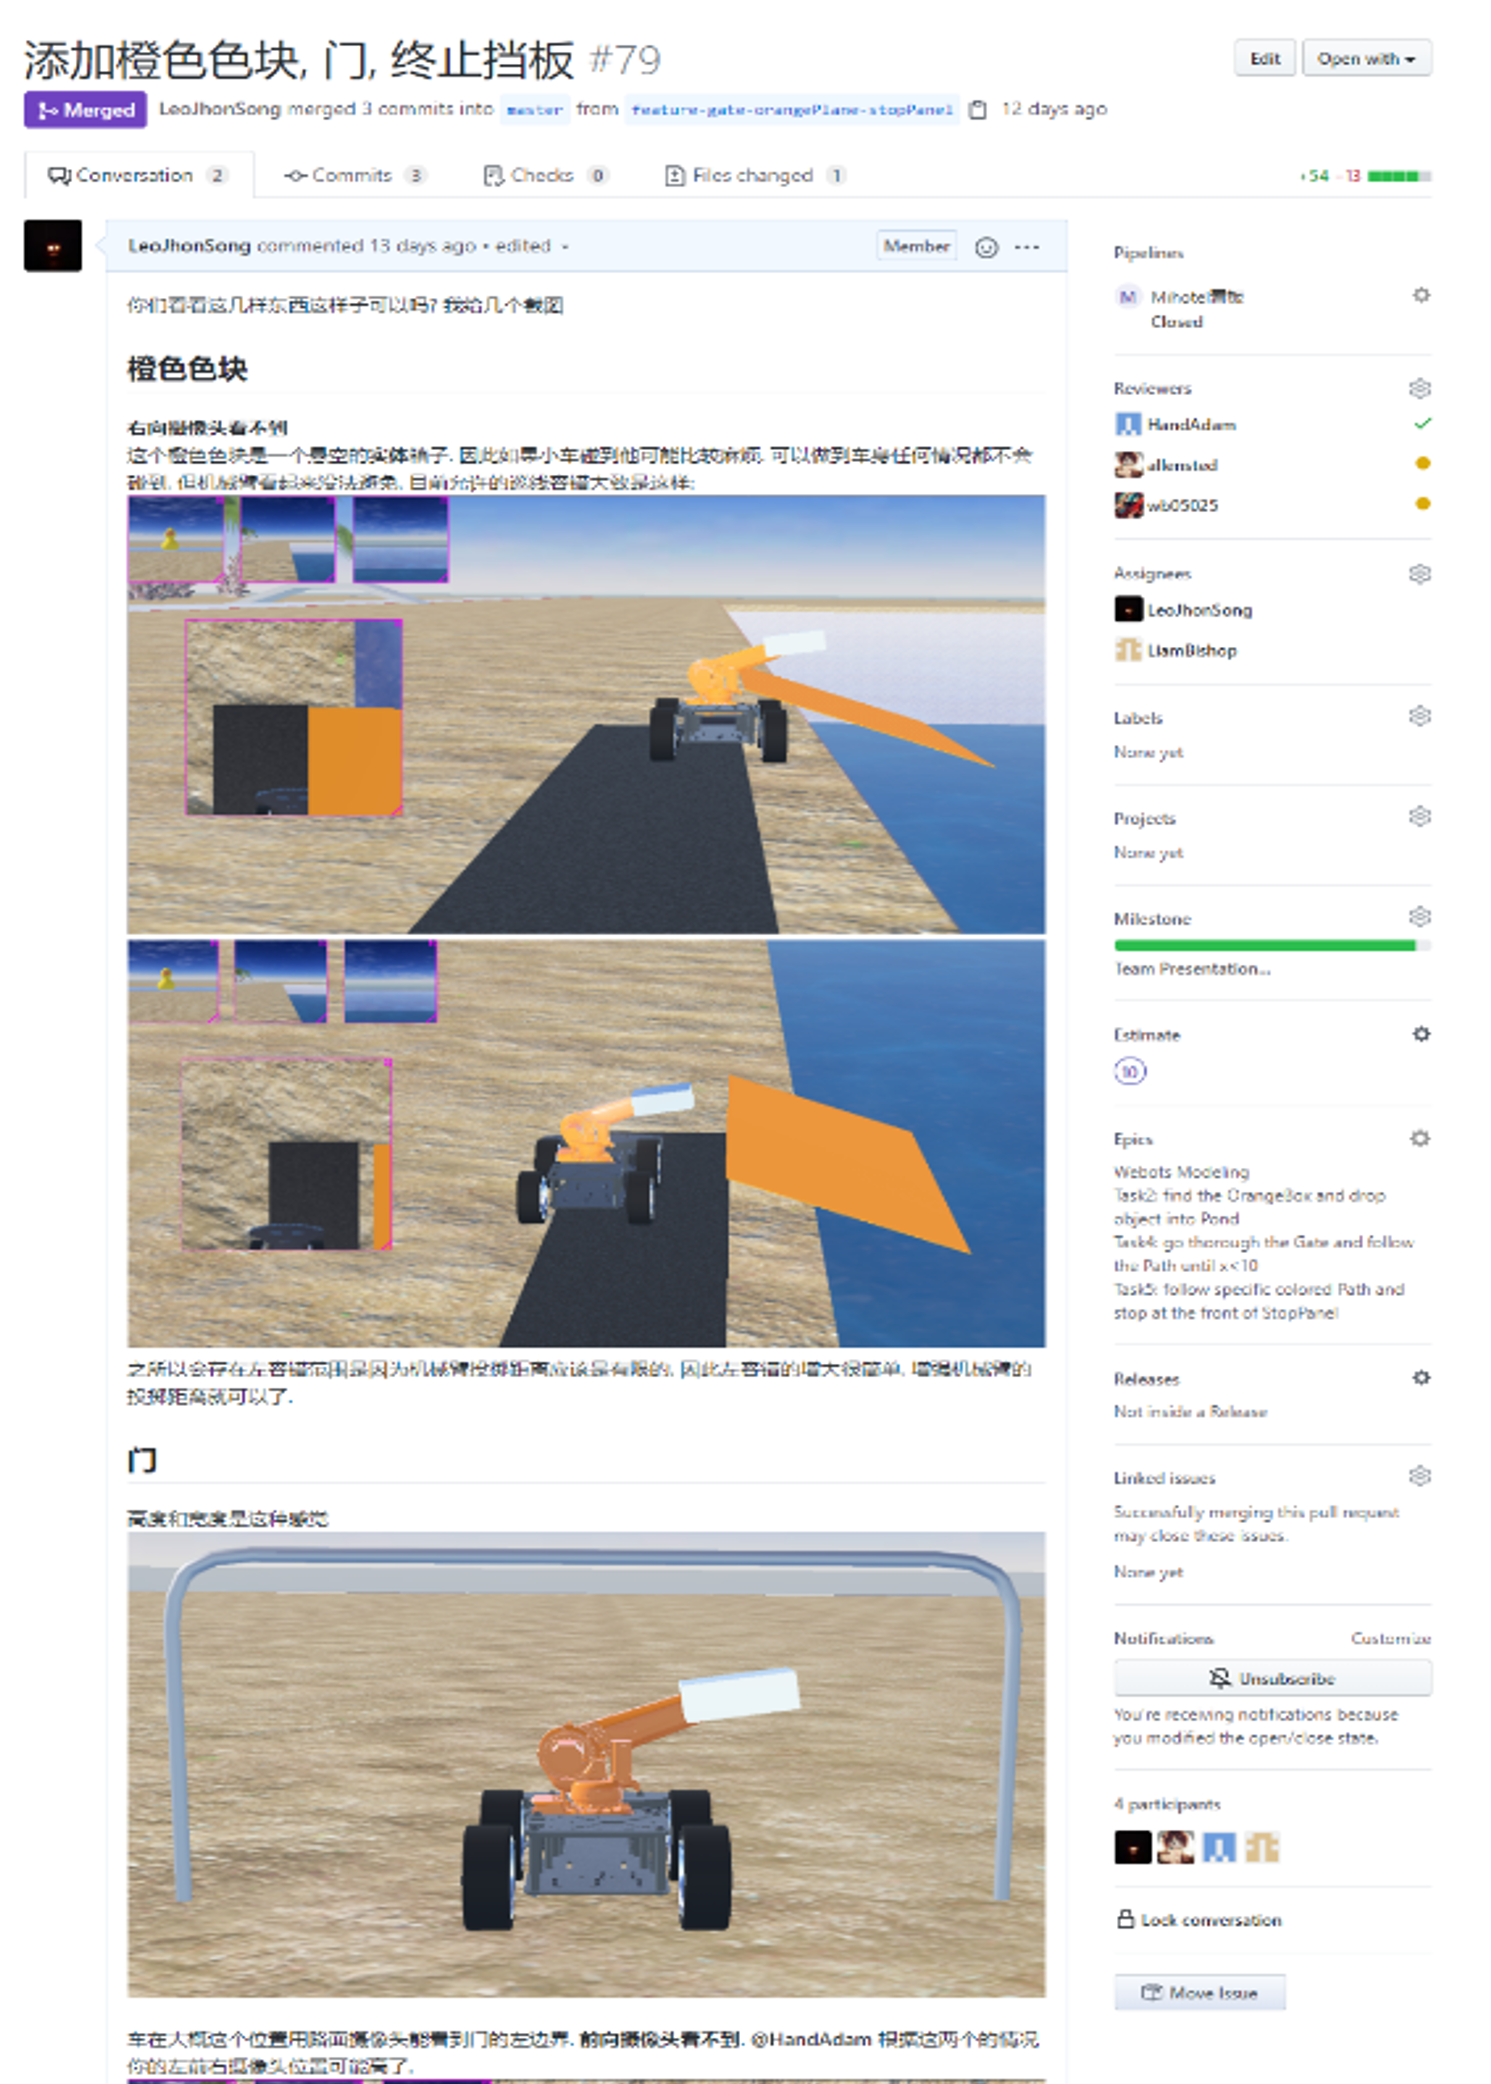
\includegraphics[width=14cm]{management/img_management/issue.png}
    \caption{Discussion board of issues}
    \label{fig:issue}
\end{figure}
%-----------------------------------------------------------------------